\documentclass[11pt,a4paper]{article}
\usepackage[margin=28mm,top=24mm,bottom=26mm]{geometry}
\usepackage{fontspec}
\IfFontExistsTF{TeX Gyre Termes}{\setmainfont{TeX Gyre Termes}}{\setmainfont{Times New Roman}}
\IfFontExistsTF{TeX Gyre Heros}{\setsansfont{TeX Gyre Heros}}{\setsansfont{Arial}}
\IfFontExistsTF{TeX Gyre Cursor}{\setmonofont{TeX Gyre Cursor}[Scale=0.85]}{\setmonofont{Courier New}[Scale=0.85]}
\usepackage{microtype,amsmath,booktabs,tabularx,graphicx,caption}
\usepackage[authoryear,round]{natbib}
\usepackage{tikz}
\usetikzlibrary{arrows.meta,positioning}
\usepackage[hidelinks]{hyperref}
\hypersetup{pdftitle={Magda: From Supermarket Flyers to Structured Offers},
  pdfauthor={Bogdan Roth, Kjell Lavezzari, Noah Samel},
  pdfsubject={Information Extraction, Summer Semester 2026}}
\setlength{\parindent}{0pt}
\setlength{\parskip}{5pt plus 1pt minus 1pt}
\linespread{1.04}
\setlength{\emergencystretch}{2em}
\setlength{\tabcolsep}{5pt}
\renewcommand{\arraystretch}{1.15}
\captionsetup{font=small,labelfont=bf,skip=7pt}
\setlength{\textfloatsep}{16pt plus 3pt minus 3pt}
\renewcommand{\topfraction}{.9}
\renewcommand{\bottomfraction}{.8}
\renewcommand{\textfraction}{.08}
\renewcommand{\floatpagefraction}{.8}
\setcounter{totalnumber}{6}
\setcounter{topnumber}{4}
\setcounter{bottomnumber}{4}
\newcommand{\entity}[1]{\textsf{\small #1}}
\newcommand{\file}[1]{{\small\nolinkurl{#1}}}
\newcommand{\tabnote}[1]{\par\vspace{3pt}{\footnotesize #1\par}}
\title{\vspace{-1.3em}Magda: From Supermarket Flyers\\to Structured Offers}
\author{Bogdan Roth\qquad Kjell Lavezzari\qquad Noah Samel\\[4pt]
  \small Leuphana University Lüneburg\\
  \small Information Extraction, Summer Semester 2026}
\date{23 September 2026}

\begin{document}
\maketitle
\vspace{-1.3em}
\begin{abstract}
\noindent
Large language models may seem hard to beat at extracting information from documents. But using an external API for every document can become costly. We wanted to find out whether smaller models adapted to a specific task could achieve comparable results locally. Magda turns flyers from the German supermarket chain PENNY into structured offers by finding product details and linking those that belong together. For our Information Extraction seminar, we followed our project proposal by using Claude Sonnet 5 to label 666 pages with 33,457 entity spans. We used the training split to fine-tune GBERT, XLM-R, LiLT and LayoutXLM on remote GPUs, comparing models using text, word positions and page images. We also trained a multilayer perceptron to predict whether two entities belong to the same offer based on entity types, spatial relations and lexical features. We compare this learned grouping approach with a rule-based heuristic and evaluate Union-Find and integer linear programming for constructing offer groups. On 42 pages with human annotations, Magda matches 212 of 279 reference records among 281 predictions and achieves an F1 score of 0.7571 for product names and regular prices. Qwen3.8-27B returns 349 records, including some duplicates, matches 240 reference records and achieves 0.7643 F1. The 95\% paired bootstrap interval for the F1 difference includes zero, providing no clear evidence that either system performs better. Entity recognition is evaluated separately using SemEval matching schemes to distinguish exact span matches from partial overlaps and type agreement. Record F1 measures agreement on product names and regular prices rather than the correctness of complete offers. Known annotation errors and prior inspection of test pages limit the conclusions to an exploratory comparison.
\end{abstract}
\begin{quote}\small
\textit{Keywords:} information extraction, document understanding, supermarket flyers, entity recognition, relation grouping, weak supervision.
\end{quote}

\section{Introduction}
The starting point for Magda was an earlier project by one of the authors, which used the Gemini API to extract structured offers from weekly supermarket flyers. The estimated API cost in that prototype was approximately EUR~0.08 per flyer. Although this was inexpensive, the prototype required an external model call for every new document. For the Information Extraction seminar, our research question was whether a locally deployed pipeline could match the extraction quality of API-based approaches while eliminating recurring API calls. We assess this through precision, recall and F1.

The original prototype sent images of the flyer pages to Gemini and received structured offers back. For Magda, we divided this process into separate steps. PENNY flyers contain an embedded PDF text layer, so PyMuPDF can extract words and their positions without an OCR step. During fine-tuning, the recognition models learn to label each extracted word as part of a product name, price, quantity or another offer field, or as outside these categories. GBERT and XLM-R use only the word sequence. LiLT also uses the words' positions on the page, while LayoutXLM additionally receives the page image.

Recognising these fields is only part of the task. A flyer page contains several offers, and a price must be assigned to the correct product. Some offers also contain multiple variants or different prices depending on purchase conditions. Magda therefore includes a separate grouping step after recognition, combining the identified entities into offer records. This separation allows us to examine whether an error comes from recognising a field or assigning it to an offer.

Manual annotation was our first approach, but it proved too time-consuming to prepare enough training data within the project timeframe. To build a larger dataset, we used Claude Sonnet 5, a vision-capable large language model, to annotate the flyer pages. The resulting dataset contains 666 pages with 33,457 entity spans. The recognition models were fine-tuned on its training split and evaluated against a separate human-annotated reference.

Following our project proposal, we aimed to build a complete local pipeline that converts flyer PDFs into structured product offers, including names, prices and quantities, using models fine-tuned on our Claude-labelled dataset. To test whether models using layout information improve entity extraction, the evaluation measures precision, recall and F1, compares them with text-only baselines and examines common extraction errors. We also compare the complete pipeline with direct extraction by vision-language models and discuss the trade-offs in extraction quality, cost and local versus API-based processing. Our grouping experiments extend these objectives by examining how recognised entities can be assembled into offer records. Appendix~\ref{app:proposal} summarises how the implementation relates to the proposal.

\section{Background and Related Work}\label{sec:related}
The Information Extraction course covers rules, learned entity recognition and extraction from document images \citep[Weeks 3--9]{iecourse2026}. Magda applies these ideas to supermarket offers. Our proposal took \citet{akbik2018} as its course reference for sequence labelling and LayoutLM \citep{xu2020} as the starting point for using document layout.

\subsection{Entity recognition}
Week 5 introduces sequence labelling as assigning labels to tokens, including the boundaries of entities spanning several words \citep[pp.~7--8]{iecourse2026}. For Magda, this means recognising ``Frische Butter'' as one product name. \citet{akbik2018} propose contextual string embeddings, which represent words through character-level language models and their surrounding text. The authors report improvements on sequence labelling tasks, including named entity recognition.

Week 8 presents pretrained transformers and fine-tuning for token classification \citep[pp.~18--21]{iecourse2026}. Magda uses this approach with GBERT, the German BERT model introduced by \citet{chan2020}, and XLM-R, the multilingual model presented by \citet{conneau2020}. Both are adapted to our offer labels and serve as baselines using text alone.

\subsection{Document layout and images}\label{sec:layout-models}
Week 9 illustrates how converting a page into plain text can lose spatial relationships \citep[p.~7]{iecourse2026}. In a flyer, these relationships can help distinguish neighbouring offers. \citet{xu2020} propose LayoutLM to learn from text and page layout. \citet{xu2022xfund} present LayoutXLM for multilingual documents using text, layout and images. \citet{wang2022} propose LiLT, whose layout component can be combined with pretrained text models for different languages. In Magda, LiLT uses text and word positions, while LayoutXLM also receives the page image. On flyers, coordinates show which words lie close together. Images additionally capture coloured price badges and product photographs, which may help distinguish offer fields.

\subsection{Relations and structured outputs}
The course distinguishes recognising entities from identifying their relationships \citep[Week 1, p.~12]{iecourse2026}. Similarly, \citet{xu2022xfund} evaluate both entity recognition and key-value relations on XFUND. Magda learns a different relation: whether two recognised fields belong to the same offer. A pair classifier supplies scores, which a decoder combines into consistent groups.

\citet{ashok2023} investigate entity extraction through instructions and examples given to a language model. Our comparison uses vision-language models to return offers directly from page images. Week 10 discusses defining output schemas and enforcing their format \citep[pp.~6--12]{iecourse2026}. A valid JSON structure alone does not establish that the extracted product and price are correct. Magda and the external models are therefore compared against the same reference records.

\section{Data and Task Definition}\label{sec:data}
\subsection{Flyer collection and preparation}
Collecting the flyers first required identifying the PDF download URLs behind PENNY's online catalogue viewer. The collection script queried PENNY's store API, which provided links to the current flyers. These links contained catalogue IDs. Using these IDs and the URL pattern for individual pages, the downloader could retrieve the PDFs automatically.

To collect more training material within the project timeframe, we included regional editions of the weekly flyers. These editions contain differences such as regional products or changed product descriptions, providing additional examples without having to wait for another publication week.

Duplicate filtering used two stages. First, pages with identical extracted word lists were detected. For nearly identical pages, regional print codes were excluded from the comparison because these can differ even when the offer content is unchanged. The remaining words were compared using Jaccard similarity, calculated as the number of distinct words shared by both pages divided by the number appearing on either page. Pages with a similarity of at least 0.95 were linked into duplicate groups. One representative page per group was normally retained, while existing human annotations were protected.

The text acquisition stage discussed in Week 2 \citep[pp.~4--5]{iecourse2026} is handled through PDF text extraction. PENNY's PDFs contain embedded text, so no OCR is required. PyMuPDF extracts each word with a bounding box, a rectangle describing its position on the page. Page images are also saved for models that use visual input. Extraction can still produce missing words or an incorrect reading order.

\subsection{Annotation and data splits}
Claude Sonnet 5 received each page image, a numbered list of the extracted words and definitions of the entity types in Table~\ref{tab:schema}. It returned labelled spans with start and end positions in the word list. Validation rejected spans with invalid word indices or unknown entity types. Rule-based corrections shortened spans at separators such as ``oder'' and removed price or quantity annotations that contained no digits. The remaining spans were converted into BIO tags for training.

Separate Claude annotations recorded which entities belonged to the same offer. These groups provided training examples for the grouping model.

\begin{table}[htbp]
\centering\small
\caption{Entity schema. The scored record projection uses BRAND, PRODUCT and regular PRICE. The remaining types still belong to the recognition task.}\label{tab:schema}
\begin{tabularx}{\linewidth}{@{}lX@{}}
\toprule Type & Meaning \\ \midrule
\entity{PRODUCT} & Product description, including annotated variants \\
\entity{BRAND} & Brand name \\
\entity{PRICE} & Current regular price without an app condition \\
\entity{OLD\_PRICE} & Former or crossed-out comparison price \\
\entity{APP\_PRICE} & Price conditional on app use \\
\entity{QUANTITY} & Amount, weight, volume or item count \\
\entity{UNIT\_PRICE} & Unit price, for example per kilogram \\
\entity{DISCOUNT} & Explicit discount statement \\
\entity{VALID} & Validity period \\
\bottomrule
\end{tabularx}
\end{table}

The resulting dataset contains 666 pages with 33,457 labelled entity spans. The fixed split assigns 494 pages to training, 56 to development and 116 to testing. Training pages were used to fine-tune the recognition models, and development pages to select checkpoints. Test pages were used for evaluation.

The main comparison uses 42 test pages selected to represent groups of similar pages. Human annotations of both entities and offer groups provide the reference, so the evaluation goes beyond agreement with the automatic labels. Some reference annotations were based on human-reviewed AI suggestions. The pages were not systematically annotated by two independent people.

For evaluation, the brand and product descriptions within each group form the offer name. Each distinct regular price produces one record with that name and price. Groups without a usable name or regular price are excluded from record scoring.

\section{Methods}\label{sec:methods}
\subsection{Pipeline overview}
Figure~\ref{fig:pipeline} shows how Magda processes a flyer page. First, a recognition model identifies product details, for example ``Frische Butter'' as PRODUCT, ``250 g'' as QUANTITY and ``1.29'' as PRICE. A separate model scores pairs of entities according to whether they belong to the same offer. A decoder then uses these scores to form groups, linking product descriptions with their prices and other details. For comparison, vision-language models receive the page images and return structured offers directly as JSON.

\begin{figure}[htbp]
\centering
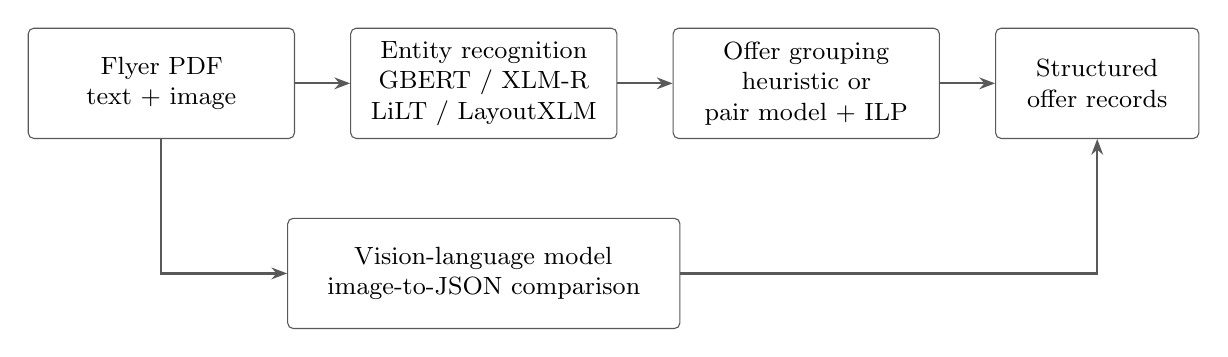
\begin{tikzpicture}[font=\small,node distance=7mm,
  box/.style={draw=black!65,rounded corners=2pt,align=center,text width=31mm,minimum height=14mm,inner sep=4pt},
  arrow/.style={-{Stealth[length=2mm]},thick,draw=black!65}]
\node[box] (pdf) {Flyer PDF\\text + image};
\node[box,right=of pdf] (ner) {Entity recognition\\GBERT / XLM-R\\LiLT / LayoutXLM};
\node[box,right=of ner] (group) {Offer grouping\\heuristic or\\pair model + ILP};
\node[box,right=of group,text width=23mm] (out) {Structured\\offer records};
\node[box,below=10mm of ner,text width=47mm] (llm) {Vision-language model\\image-to-JSON comparison};
\draw[arrow] (pdf) -- (ner); \draw[arrow] (ner) -- (group); \draw[arrow] (group) -- (out);
\draw[arrow] (pdf.south) |- (llm.west); \draw[arrow] (llm.east) -| (out.south);
\end{tikzpicture}
\caption{Inference paths. LayoutXLM uses the page image as well as words and positions. All local entity outputs remain anchored to extracted words. LLM-assisted training annotation is a separate, earlier process.}\label{fig:pipeline}
\end{figure}

\subsection{Entity recognition}
Entity recognition assigns a label to each extracted word. Following the BIO scheme covered in Week 5 \citep[p.~8]{iecourse2026}, ``Frische'' receives B-PRODUCT and ``Butter'' receives I-PRODUCT. B marks the beginning of an entity, I its continuation, and O a word outside the defined entity types. This allows the model to recognise a product name that spans several words.

The four models use different inputs. GBERT and XLM-R receive text, LiLT also receives word positions, and LayoutXLM additionally receives the page image. Each model's pretrained encoder turns its input into numerical representations that include context. A classification layer uses these representations to predict BIO labels. During fine-tuning, both the encoder and this layer are adjusted using our labelled pages, following the approach discussed in Week 8 \citep[p.~21]{iecourse2026}. The training procedure selects the checkpoint with the highest development F1.

Tokenisation can split a word into several smaller pieces. Only the first piece receives the word's training label. The remaining pieces stay in the input but are excluded from the loss calculation, so a word is not counted several times simply because it was split. During training, inputs exceeding the model's length limit are truncated. At inference, overlapping windows allow longer pages to be processed and their predictions combined.

\subsection{Pairwise offer membership}\label{sec:pair-features}
For grouping, we compared a rule-based heuristic with a multilayer perceptron (MLP). The heuristic first groups nearby descriptive fields and price badges separately. It then links these groups using quantity times unit price where possible, and spatial proximity otherwise.

The final MLP uses 43 numerical features per entity pair. \emph{Base} combines entity-type indicators with distances, bounding-box overlap, text height and position in the word sequence. \emph{Extended geometry}, called Geometry in Table~\ref{tab:features}, describes nearby alternatives and intervening product names or words. For example, another product closer to a price may be a better match. \emph{Lexical} features indicate words such as ``je'' or ``Aktion'' before an entity, or ``oder'' between entities. These are inputs whose influence the MLP learns, rather than fixed grouping rules.

Additional variants tested \emph{anchor} and \emph{colour} features. Anchor features indicate whether both entities share the same nearest product or brand name as a reference point, and their distances to their respective anchors. Colour features compare the entities' backgrounds and colour continuity along the line between them. Neither block is included in the final model.

The MLP combines these inputs through two hidden layers with 64 and 32 units and ReLU activations. These nonlinear layers allow combinations of features to influence the prediction. Training pairs from the same Claude-annotated offer are labelled positive, while pairs from different offers are labelled negative. Training adjusts the network's weights to reduce prediction errors on these examples. A sigmoid function converts its output into a score between zero and one, which the decoder uses to construct offer groups.

\subsection{Consistent groups through structured decoding}
We compared two methods for turning pair scores into offer groups. Using Union-Find \citep{tarjan1975}, entities are merged when their pair score meets a threshold. This also creates indirect links. If A is linked to B and B to C, all three form one group. An incorrect link can therefore combine separate offers.

The second method uses integer linear programming (ILP), following the clustering formulation studied by \citet{groetschel1989}. It weighs supporting and conflicting pair scores together when choosing groups. This allows it to reject a connection that would otherwise join poorly matching entities. For very large candidate groups, our implementation retains the Union-Find result to limit computation.

The choice was practical. Union-Find provided a simple baseline, while ILP achieved better exact group matching in our earlier comparison against automatically annotated offer groups (Section~\ref{sec:grouping-results}).

\subsection{Direct extraction with vision-language models}
Gemma-4-31B-IT, Qwen3.6-35B-A3B and Mistral-Medium-3.5-128B were selected from the vision-language models available to us through Academic Cloud. Each received images of the same 42 test pages and a prompt specifying the offer fields and JSON format. They were not fine-tuned for this project. A later run added Qwen3.8-27B through the TH L\"ubeck API, using the same extraction prompt with thinking disabled.

GPT-6 Astra was evaluated separately in a fresh Codex conversation with reasoning effort set to \texttt{high}, using the same images and extraction instructions. The model was instructed to use only these inputs and save each page's JSON output before evaluation. Unlike the separate API requests, this run retained context across pages and used tools to view images and save files. We therefore report it as a supplementary comparison. Since the direct outputs do not provide aligned entity spans, all systems are compared on product names and regular prices against the same human reference.

Processing time was measured for Magda and Qwen3.8-27B, with pages processed sequentially. PDF download, text extraction and image rendering were completed beforehand. Local model loading was recorded separately, and an additional warm-up run was excluded from timing. Magda ran on the local macOS machine. API times include network and server delays, and the remote hardware was not controlled. These timings describe the tested setup and exclude the Codex run.

\section{Experimental Design and Evaluation}\label{sec:evaluation}
\subsection{Evaluation setup}
To create the human reference, we developed a web-based annotation tool that displays the extracted words on the flyer image. Annotation followed two steps. First, entity spans such as product names, prices and quantities were labelled and reviewed manually. The labelled entities were then assigned to offer groups. This produced separate references for entity recognition and grouping on the 42 test pages.

For the grouping comparison, the rule-based heuristic and learned model receive the same human-annotated entities. The learned grouper is also evaluated on LayoutXLM predictions to include recognition errors. Finally, Magda and the vision-language systems are compared on product names and regular prices. Earlier feature and decoder experiments use automatically annotated groups as their reference and are reported separately.

\subsection{Evaluation metrics}
Precision ($P$) is the proportion of predictions that match the reference. Recall ($R$) is the proportion of reference items recovered. F1 combines both:
\begin{equation}
 F_1=\frac{2PR}{P+R}.
\end{equation}
Counts are pooled across pages before calculating micro-F1.

Entity recognition uses the SemEval matching schemes \citep{segura2013}. \emph{Strict}, our primary metric, requires exact word boundaries and the correct entity type. \emph{Exact} checks boundaries only. \emph{Partial} ignores type and gives full credit for exact boundaries or half credit for an overlapping span. \emph{Type} requires the correct type and at least one overlapping word. Thus, predicting ``Butter'' instead of ``Frische Butter'' fails Strict but can receive Partial or Type credit.

Pair F1 measures whether entity pairs share an offer as in the reference. Large groups contribute more pairs. Exact group F1 requires the complete set of matched entities to agree, so one missing or additional entity can invalidate a group. Unmapped entities are reported separately.

A predicted record matches a reference record if their regular prices are identical and their names reach a character-based similarity score of at least 0.6 on a scale from 0 to 1. This cutoff was chosen to allow differences in wording and was not calibrated as an optimal value. The assignment maximises the number of matches while counting each prediction and reference record at most once. Records without a usable name or regular price are excluded from both predictions and reference. Failed external responses count as empty outputs. Record F1 covers product names and regular prices. Other fields, such as quantity and app conditions, are outside this score.

\subsection{Uncertainty and interpretation}
A small F1 difference may depend on which pages are evaluated. To examine this uncertainty, we use a paired bootstrap, a resampling approach discussed by \citet{dror2018}. Each resample draws 42 times from the 42 test pages, with replacement. Some pages therefore appear several times, while others are absent. For example, three pages $A,B,C$ could be resampled as $A,A,C$. The sample size stays constant, but $A$ counts twice and $B$ does not contribute. Both systems receive exactly the same selection. Their saved outputs are used to recompute pooled F1 and the difference between systems, without retraining or new model requests.

The 42 pages each represent a different template cluster, formed using word-set Jaccard similarity at a threshold of 0.7. This lower cutoff groups broader regional variants, whereas duplicate filtering at 0.95 targets nearly identical content. Both cutoffs were chosen heuristically and were not calibrated as optimal values. Selecting one page per cluster limits repeated regional variants but does not guarantee independence. The percentile bootstrap uses 10,000 resamples with seed 42. It estimates uncertainty from the available pages and does not provide new test data.

An unadjusted 95\% interval spans the middle 95\% of the resampled F1 differences. Bonferroni-adjusted intervals account for multiple comparisons in two exploratory families, four recognition comparisons and three original API comparisons against Magda. The later Qwen3.8 and Astra comparisons are reported separately. An interval that includes zero establishes neither a clear winner nor equivalence. These intervals describe resampling of fixed outputs and labels, excluding uncertainty from annotation errors, retraining or repeated model requests.

\section{Results and Error Analysis}\label{sec:results}
\subsection{Entity recognition}
Strict F1 is similar across the four models on 42 human-annotated pages (Table~\ref{tab:ner}). LayoutXLM scores highest, but all adjusted paired intervals include zero (Appendix~\ref{app:tables}). Thus, LiLT and LayoutXLM from Section~\ref{sec:layout-models} show no clear advantage over the text-only baselines here. Different pretraining also prevents isolating the effect of layout or images.

\begin{table}[htbp]
\centering\small
\caption{Entity recognition against the human reference. Scores pool counts across the 42 pages. Intervals are individual 95\% cluster intervals.}\label{tab:ner}
% Automatisch aus gespeicherten Ergebnissen erzeugt.
\begin{tabular}{@{}lrrrl@{}}
\toprule
Model & Precision & Recall & Strict F1 & 95\% CI \\
\midrule
GBERT & 0.7053 & 0.7010 & 0.7032 & $[0.6390,\,0.7556]$ \\
XLM-R & 0.7157 & 0.7071 & 0.7114 & $[0.6473,\,0.7651]$ \\
LiLT & 0.7066 & 0.6961 & 0.7013 & $[0.6379,\,0.7537]$ \\
LayoutXLM & 0.7210 & 0.7131 & 0.7170 & $[0.6514,\,0.7716]$ \\
\bottomrule
\end{tabular}

\end{table}

\begin{table}[htbp]
\centering\small
\caption{Strict F1 by entity type on the same 42 human-annotated pages. Both word boundaries and entity type must match. The reference count gives the number of annotated entities of each type.}\label{tab:entity-scores}
% Automatisch aus gespeicherten Ergebnissen erzeugt.
\begin{tabular}{@{}lrrrrr@{}}
\toprule
Entity type & Reference spans & GBERT & XLM-R & LiLT & LayoutXLM \\
\midrule
APP\_PRICE & 62 & 0.7368 & 0.6078 & 0.5657 & 0.5743 \\
BRAND & 254 & 0.8612 & 0.8800 & 0.8737 & 0.9138 \\
DISCOUNT & 140 & 0.9474 & 0.9474 & 0.9474 & 0.9333 \\
OLD\_PRICE & 120 & 0.8537 & 0.8816 & 0.8468 & 0.8908 \\
PRICE & 291 & 0.8643 & 0.8719 & 0.8586 & 0.8826 \\
PRODUCT & 322 & 0.5208 & 0.5385 & 0.5310 & 0.5651 \\
QUANTITY & 337 & 0.3711 & 0.3726 & 0.3662 & 0.3639 \\
UNIT\_PRICE & 255 & 0.7787 & 0.7802 & 0.7802 & 0.7802 \\
VALID & 42 & 0.8293 & 0.9024 & 0.8675 & 0.8000 \\
\bottomrule
\end{tabular}

\end{table}

The larger differences are between entity types (Table~\ref{tab:entity-scores}). Product names and quantities are harder to match exactly than regular and old prices. Every model scores below 0.38 on QUANTITY, despite this being the most frequent reference type. The error analysis below shows how inconsistent span boundaries contribute to this problem.

For LayoutXLM, changing the matching scheme raises F1 from 0.7170 under Strict to 0.8720 under Type. The predictions are unchanged. Type accepts overlapping spans with the correct label, so this gap shows how much the result depends on requiring exact boundaries. Appendix~\ref{app:tables} reports all four matching schemes.

\subsection{Grouping and component experiments}\label{sec:grouping-results}
On the same human-annotated entities, learned grouping increases exact group F1 from 0.4164 to 0.7112 (Table~\ref{tab:grouping}). Because both methods receive identical fields, this difference comes from assigning them to offers. Pair F1 is higher than exact group F1 for both methods. Many individual links can be correct while one missing or additional entity still makes the complete group fail.

\begin{table}[htbp]
\centering\small
\caption{All rows are evaluated against human-annotated offer groups. The first two use identical human-annotated entities and compare grouping alone. The third uses LayoutXLM predictions. Unmapped entities cannot be assigned to the grouping reference. Intervals are individual 95\% intervals, with no separate paired test.}\label{tab:grouping}
% Automatisch aus gespeicherten Ergebnissen erzeugt.
\begin{tabular}{@{}l>{\raggedright\arraybackslash}p{29mm}rrlr@{}}
\toprule
Grouping method & Entity input & Pair F1 & Group F1 & 95\% CI (group) & Unmapped \\
\midrule
Rule-based & Human-annotated entities & 0.7291 & 0.4164 & $[0.3094,\,0.5329]$ & 49 \\
MLP + ILP & Human-annotated entities & 0.9168 & 0.7112 & $[0.5977,\,0.8090]$ & 49 \\
MLP + ILP & LayoutXLM predictions & 0.9267 & 0.7264 & $[0.6197,\,0.8180]$ & 212 \\
\bottomrule
\end{tabular}

\end{table}

Using predicted entities gives a slightly higher conditional grouping score, but unmapped entities increase from 49 to 212. The set of evaluable pairs changes with the input. This higher score therefore does not mean that recognition errors improve grouping. The record comparison below includes their effect on the final output.

Earlier experiments helped us choose the grouping features. Each variant was trained on 494 pages, with the classifier architecture and ILP decoder held fixed and its threshold calibrated on training folds. The reference consisted of automatically generated groups. Adding extended geometry and lexical cues gave the highest exact group F1 in this comparison (Table~\ref{tab:features}). This gain belongs to the combined feature set, so it cannot be attributed to lexical cues alone. Adding anchor features to that combination reduced the score. More features did not automatically help.

\begin{table}[htbp]
\centering\footnotesize
\caption{Earlier feature comparison on 56 development pages in 25 clusters, against automatic annotations. Each variant was retrained and calibrated. Difference intervals use 1,000 bootstrap resamples without correction for multiple comparisons.}\label{tab:features}
% Automatisch aus gespeicherten Ergebnissen erzeugt.
\begin{tabular}{@{}lrrrl@{}}
\toprule
Feature set & Count & Group F1 & $\Delta$ vs. base & 95\% CI \\
\midrule
Base & 30 & 0.7017 & -- & -- \\
Base + colour & 34 & 0.7454 & $+0.0437$ & $[+0.0127,\,+0.0750]$ \\
Base + geometry & 35 & 0.7779 & $+0.0762$ & $[+0.0276,\,+0.1422]$ \\
Base + geometry + colour & 39 & 0.7981 & $+0.0964$ & $[+0.0356,\,+0.1671]$ \\
Base + geometry + anchor & 38 & 0.7834 & $+0.0817$ & $[+0.0164,\,+0.1484]$ \\
Base + geometry + lexical & 43 & 0.8206 & $+0.1189$ & $[+0.0577,\,+0.1842]$ \\
Base + geometry + anchor + lexical & 46 & 0.7778 & $+0.0761$ & $[+0.0327,\,+0.1280]$ \\
\bottomrule
\end{tabular}

\tabnote{Feature blocks are explained in Section~\ref{sec:pair-features}. Base contains entity types and base geometry. Geometry denotes the additional spatial context. Count is the number of input features.}
\end{table}

A separate earlier decoder experiment used 75 pages in 68 clusters, evaluated out of fold against automatic groups. With separately calibrated thresholds, ILP increased exact group F1 from 0.4526 to 0.5530, while pair F1 fell from 0.7153 to 0.5694. The procedures were calibrated for exact group F1, and the two metrics favoured different outcomes. The group F1 difference had an unadjusted 95\% interval of $[+0.0668,+0.1332]$ from 1,000 bootstrap resamples. This compares decoding together with calibration. The saved run includes fallback for large components and lacks a complete page inventory, which limits its reproducibility.

\subsection{Complete pipeline and model comparison}\label{sec:record-results}
Magda matches 212 of 279 reference records among 281 outputs (Table~\ref{tab:offers}). Qwen3.8 matches more reference records, but also returns more outputs without a match, giving it higher recall and lower precision. Their F1 scores are close because F1 combines both. An unmatched output can reflect an extraction error, a different offer boundary or a problem in the reference.

\begin{table}[htbp]
\centering\small
\caption{Product-name and regular-price matching on the same 42 pages and 279 reference records. The later API and Codex runs are separated from the original comparison.}\label{tab:offers}
% Automatisch aus gespeicherten Ergebnissen erzeugt.
\begin{tabular}{@{}lrrrrr@{}}
\toprule
System & Matches & Outputs & Precision & Recall & F1 \\
\midrule
Magda & 212 & 281 & 0.7544 & 0.7599 & 0.7571 \\
Gemma-4-31B-IT & 200 & 272 & 0.7353 & 0.7168 & 0.7260 \\
Qwen3.6-35B-A3B & 231 & 328 & 0.7043 & 0.8280 & 0.7611 \\
Mistral-Medium-3.5-128B & 207 & 340 & 0.6088 & 0.7419 & 0.6688 \\
\midrule
Qwen3.8-27B (later API run) & 240 & 349 & 0.6877 & 0.8602 & 0.7643 \\
\midrule
GPT-6 Astra (Codex) & 241 & 315 & 0.7651 & 0.8638 & 0.8114 \\
\bottomrule
\end{tabular}

\tabnote{Gemma had five pages without usable responses and Mistral three, counted as empty outputs. Astra used a shared Codex conversation with high reasoning, rather than separate API requests.}
\end{table}

The supplementary Astra run has the highest F1 point estimate. It matches one more reference record than Qwen3.8 with fewer outputs, giving it higher precision. Its shared conversation and tool use differ from the API setup, so this is an additional comparison under different conditions.

For the comparison model's F1 minus Magda's F1, the paired 95\% interval is $[-0.0759,+0.1110]$ for Qwen3.8 and $[-0.0308,+0.1547]$ for Astra. Negative values favour Magda, positive values favour the comparison model. Both ranges cross zero and include sizeable differences in either direction. The available pages therefore establish neither a clear winner nor equivalent performance. The original API intervals also include zero before and after correction (Appendix~\ref{app:tables}). The later intervals are exploratory and separate from the original comparison family.

The score excludes 22 reference fragments, 106 Magda fragments and six Qwen3.8 fragments without a usable name or regular price. It therefore describes matching on those two fields, rather than the proportion of complete offers extracted correctly.

Processing prepared pages took Magda an average of 0.695 seconds per page, compared with 26.965 seconds for Qwen3.8 through the TH L\"ubeck API. Local model loading took 4.439 seconds separately. Magda was faster in this setup. PDF preparation was excluded, and Qwen's time includes network and server delays on uncontrolled remote hardware. No comparable timing was recorded for Astra.

\subsection{Error analysis}\label{sec:error-results}
Boundary and merge deviations were the most frequent category among reference entities without an exact match. Table~\ref{tab:examples} illustrates why these disagreements need inspection. Some concern span definitions, while others change the product-price association or originate in the reference itself.

\begin{table}[htbp]
\centering\small
\caption{Examples from catalogue 1364390, based on saved span diagnostics and the exploratory visual review.}\label{tab:examples}
\begin{tabularx}{\linewidth}{@{}>{\raggedright\arraybackslash}p{2.4cm}X@{}}
\toprule Case & Observation and consequence \\ \midrule
Span boundary, p.~1 & LayoutXLM predicts ``500 g'' as one QUANTITY span. The reference stores ``500'' and ``g'' separately. The amount is recognisable, but the spans fail Strict matching. \\
Wrong price, p.~22 & Magda assigns 3.49 to Philadelphia cream cheese instead of the displayed 2.29. Recognising the product alone does not produce a correct record. \\
Duplicate, p.~21 & Qwen3.8 returns ``Tempo Taschent\"ucher'' at 2.99 twice. A reference record can match only one of these outputs. \\
Reference error, p.~3 & The regular price 2.69 after ``ohne PENNY App'' is labelled OLD\_PRICE. If its group has no PRICE, it produces no scored reference record. \\
\bottomrule
\end{tabularx}
\end{table}

A separate review checked every scored Magda and Qwen3.8 output against its page image. It identified ten Qwen duplicates, while many additional outputs represented visible offers or variants. This was a single AI review of emitted records, not an independent human reference or a check of all missed offers. The original annotations and reported scores remain unchanged.

\section{Discussion}\label{sec:discussion}
The four recognition models achieved similar overall scores, leaving no clear architectural winner for local field recognition. Learned grouping improved the assignment of the same human-annotated entities compared with fixed rules. For Magda, this highlights the importance of both stages: recognising a price and linking it to the right product. In the earlier feature experiments, combining additional spatial context and lexical cues gave the best grouping result against automatic annotations. Adding anchor features reduced the score. More input features did not automatically make the model better.

The complete pipeline addresses our original question more directly. For product names and regular prices, Magda ran locally and reached F1 scores close to Qwen (Table~\ref{tab:offers}). Qwen3.8 recovered more reference records, while Magda had fewer unmatched outputs relative to its total output. Some additional Qwen records were duplicates, while others appeared to be valid offers or variants. Astra scored highest in the separate Codex run, which used shared context and tools. The paired intervals against Magda leave the ranking uncertain, and similar scores do not prove equivalent performance. A record can also fail matching because one field differs, even when other details are correct. These scores therefore give only part of the picture of practical extraction quality.

The project supports the idea that local extraction is viable for product names and regular prices on the evaluated PENNY pages. Magda reached 0.7571 F1, close to Qwen3.8's 0.7643 (Table~\ref{tab:offers}). Processing prepared pages took 0.695 seconds per page on average, versus 26.965 seconds through the Qwen3.8 API (Section~\ref{sec:record-results}). These timings reflect different hardware and network conditions. Annotation, training, maintenance and inference still require resources. The comparison does not show that the pipeline is free or cheaper than using an API overall.

\section{Limitations}\label{sec:limitations}
\textbf{Reference quality.} The annotations contain known errors, and decisions about span boundaries or shared prices involve judgement. Some annotations began as AI suggestions that were reviewed manually. There was no systematic independent second annotation of every page. The additional visual review used one AI reviewer and checked emitted records, so it cannot establish how many visible offers were missed.

\textbf{Data and uncertainty.} Evaluation covers 42 PENNY pages, and test pages had already been inspected during development. The results therefore remain exploratory. The pipeline requires a PDF text layer, and transfer to new weeks or retailers was not tested. The bootstrap resamples one saved output set per system. It does not measure uncertainty from annotation errors, retraining or repeated model requests.

\textbf{Comparability.} The original API comparison covered models available through Academic Cloud and was not an exhaustive benchmark. Astra used shared context and tools in Codex, so its run differs from separate API requests. The recognition models also differ in pretraining, which prevents isolating the benefit of layout or images. Earlier grouping experiments used automatic references and partly incomplete run records.

\textbf{Evaluation scope.} Record F1 covers product names and regular prices, excludes incomplete fragments and does not assess all offer conditions. Additional post-processing of the final records, such as standardising quantity formats or handling duplicate offers, was not evaluated systematically. Its benefit therefore remains unmeasured. Runtime measurements excluded PDF preparation and compared a local machine with an uncontrolled remote service, including network delays. Total operating costs were not measured.

\section{Conclusion and Outlook}\label{sec:conclusion}
We built Magda to extract offers from PENNY flyers with models that run locally. The pipeline first recognises product names, prices and other details, then decides which belong together. Evaluating these steps separately helped us understand where errors occur.

The four recognition models reached similar overall F1 scores. Learned grouping performed better than fixed rules when both used the same human-annotated entities. On the same pages, Magda reached F1 scores close to Qwen for product names and regular prices, without an external model call for each page. This supports local extraction as a feasible approach for these fields in our PENNY case study. Astra scored higher in a separate Codex run, but its setup differed. The paired comparisons with Qwen and Astra did not establish a clear winner. Similar scores also do not prove equal performance.

Magda is a working prototype and a starting point for further research. A next study could improve the annotation rules and test the pipeline on a new flyer week with independently checked labels. Additional post-processing, such as standardising quantity formats and handling duplicates, could be developed on training and development pages before testing whether it improves the final records.

\begingroup
\small
\setlength{\bibsep}{4pt}
\interlinepenalty=10000
\exhyphenpenalty=10000
\bibliographystyle{plainnat}
\bibliography{references}
\endgroup
\appendix
\section{Supplementary Results}\label{app:tables}
\captionsetup{hypcap=false}
The tables below retain the full paired comparisons from the original study. Bonferroni intervals use separate families for recognition and record reconstruction. The offer tables refer to the original Academic Cloud runs. Section~\ref{sec:record-results} reports the later Qwen3.8 and Astra comparisons. The individual intervals in Table~\ref{tab:offer-intervals} do not replace paired differences.

\begin{center}\begin{minipage}{\linewidth}
\centering\small
\captionof{table}{Recognition F1 under four matching schemes on the same human-reference pages.}
% Automatisch aus gespeicherten Ergebnissen erzeugt.
\begin{tabular}{@{}lrrrr@{}}
\toprule
Model & Strict & Exact & Partial & Type \\
\midrule
GBERT & 0.7032 & 0.7202 & 0.8066 & 0.8688 \\
XLM-R & 0.7114 & 0.7252 & 0.8082 & 0.8720 \\
LiLT & 0.7013 & 0.7184 & 0.8033 & 0.8654 \\
LayoutXLM & 0.7170 & 0.7281 & 0.8081 & 0.8720 \\
\bottomrule
\end{tabular}

\end{minipage}\end{center}

\begin{center}\begin{minipage}{\linewidth}
\centering\small
\captionof{table}{Paired recognition differences, with a family of four comparisons.}
% Automatisch aus gespeicherten Ergebnissen erzeugt.
\begin{tabular}{@{}lrll@{}}
\toprule
Comparison & $\Delta$F1 & 95\% CI & Bonferroni CI \\
\midrule
XLM-R $-$ GBERT & $+0.0082$ & $[-0.0075,\,+0.0286]$ & $[-0.0109,\,+0.0355]$ \\
LiLT $-$ XLM-R & $-0.0101$ & $[-0.0236,\,+0.0010]$ & $[-0.0275,\,+0.0031]$ \\
LayoutXLM $-$ LiLT & $+0.0157$ & $[+0.0015,\,+0.0325]$ & $[-0.0015,\,+0.0374]$ \\
LayoutXLM $-$ GBERT & $+0.0139$ & $[-0.0036,\,+0.0367]$ & $[-0.0070,\,+0.0440]$ \\
\bottomrule
\end{tabular}

\end{minipage}\end{center}

\begin{center}\begin{minipage}{\linewidth}
\centering\small
\captionof{table}{Individual intervals for record-level F1.}\label{tab:offer-intervals}
% Automatisch aus gespeicherten Ergebnissen erzeugt.
\begin{tabular}{@{}lrl@{}}
\toprule
System & F1 & 95\% CI \\
\midrule
Magda & 0.7571 & $[0.6551,\,0.8521]$ \\
Gemma-4-31B-IT & 0.7260 & $[0.6344,\,0.8088]$ \\
Qwen3.6-35B-A3B & 0.7611 & $[0.6817,\,0.8330]$ \\
Mistral-Medium-3.5-128B & 0.6688 & $[0.5842,\,0.7504]$ \\
\bottomrule
\end{tabular}

\end{minipage}\end{center}

\begin{center}\begin{minipage}{\linewidth}
\centering\small
\captionof{table}{External system minus local pipeline: paired record-level differences, with a family of three comparisons.}
% Automatisch aus gespeicherten Ergebnissen erzeugt.
\begin{tabular}{@{}>{\raggedright\arraybackslash}p{39mm}rll@{}}
\toprule
Comparison & $\Delta$F1 & 95\% CI & Bonferroni CI \\
\midrule
Gemma-4-31B-IT $-$ Magda & $-0.0312$ & $[-0.1450,\,+0.0908]$ & $[-0.1703,\,+0.1177]$ \\
Qwen3.6-35B-A3B $-$ Magda & $+0.0040$ & $[-0.0892,\,+0.1126]$ & $[-0.1067,\,+0.1376]$ \\
Mistral-Medium-3.5-128B $-$ Magda & $-0.0883$ & $[-0.2024,\,+0.0392]$ & $[-0.2225,\,+0.0685]$ \\
\bottomrule
\end{tabular}

\end{minipage}\end{center}

\small
\section{Reproducibility and Availability}
The project repository is \href{https://github.com/noahsa16/magda}{github.com/noahsa16/magda}. It is private, but we are happy to invite both of you on request so you can access the code and supporting materials. Evaluation uses saved predictions and model responses, with file hashes identifying the evaluated inputs. Instructions for rebuilding the report and repeating the main and supplementary analyses are documented in \file{docs/report/README.md}. These analyses require no new API calls. Model weights and most raw PDFs and page images are stored separately and are not included in a standard clone.

\section{Relation to the Project Proposal}\label{app:proposal}
The proposal called for trained extraction, documented entity scores, a text/layout comparison, error analysis, and an LLM comparison with an operational discussion. Magda addresses these within the stated scope, adding learned grouping and uncertainty analysis.

PENNY's text layer replaces the proposed OCR stage. Runs with Gemma, Qwen, Mistral and Astra replace the earlier Gemini prototype in the final comparison. Costs are discussed qualitatively, without a measured cost advantage.

\section{Use of AI}
Claude Sonnet 5 supplied training annotations and grouping suggestions. Vision-language models provided comparison outputs, including GPT-6 Astra in Codex. Codex also supported implementation and LaTeX typesetting. It helped formulate and revise the report in English.

\end{document}
